%!TEX root=document.tex


\subsection{Summary of Findings}
\label{sec:expt_summary}

\resolved{
\reviewer{
	It would be good to investigate the usefulness of the results for queries
with different ranges (for example: if Dq is a very large portion of D, it won’t
have a large deviation from average and thus it is not clear if the
recommended visualizations can be useful)
}
}
%The previous sections described the basic framework for \SeeDB and our suite of sharing and pruning optimizations.
% two suits of optimizations to efficiently process, we developed a basic framework and sets of pruning an sharing optimizations for \SeeDB.
Figures \ref{fig:all_opt_with_pruning}.a and \ref{fig:all_opt_with_pruning}.b show a summary of \SeeDB performance for the four 
(large) real datasets from Table \ref{tab:datasets} (BANK, DIAB, AIR and AIR10).
For each dataset, we show the latencies obtained on the ROW and COL store by the basic \SeeDB framework (NO\_OPT), 
by our sharing optimizations (SHARING), and by the combination of our sharing and pruning optimizations (COMB). 
We also show latencies for early result generation with COMB (COMB\_EARLY), where we return approximate results 
as soon as the top-$k$ visualizations have been identified.
The results in Figure \ref{fig:all_opt_with_pruning} 
use the CI pruning scheme and $k$=10. 

%We note that overall the results on the column store (not shown) are similar, with slightly faster overall performance.  The column store benefits less from the pruning optimizations on small datasets (BANK and DIAB), because it has a higher fixed per-query overhead than Postgres, which causes the additional queries run for each round of the pruning algorithm to introduce some penalty.  However, on these datasets the total runtimes are still only a few seconds or less no matter which optimizations we enable.

% (This figure shows results for ROW. Results for COL are discussed further in Section \ref{sec:sharing_and_pruning}).

% \begin{figure}[t]
% 	\centering
% 	\begin{subfigure}{0.24\linewidth}
% 		{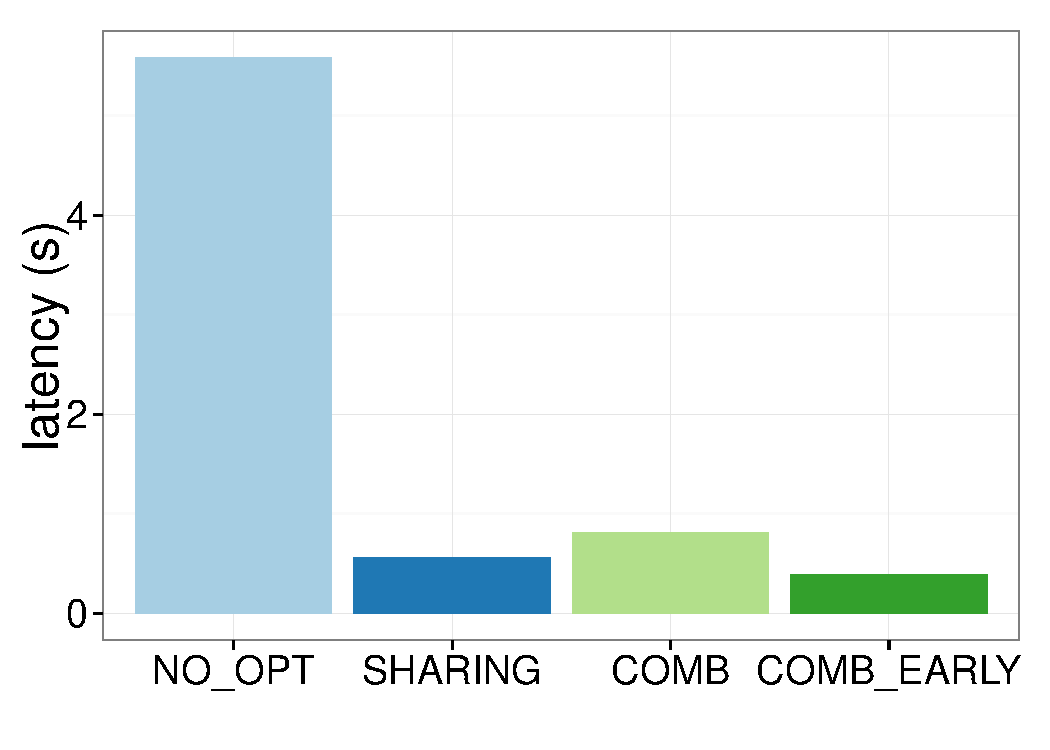
\includegraphics[width=3cm] {Images/all_opt_real_data_row_BANK.pdf}}
% 		\caption{BANK}
% 		\label{fig:baseline_size}
% 	\end{subfigure}
% 	\begin{subfigure}{0.24\linewidth}
% 		\centering
% 		{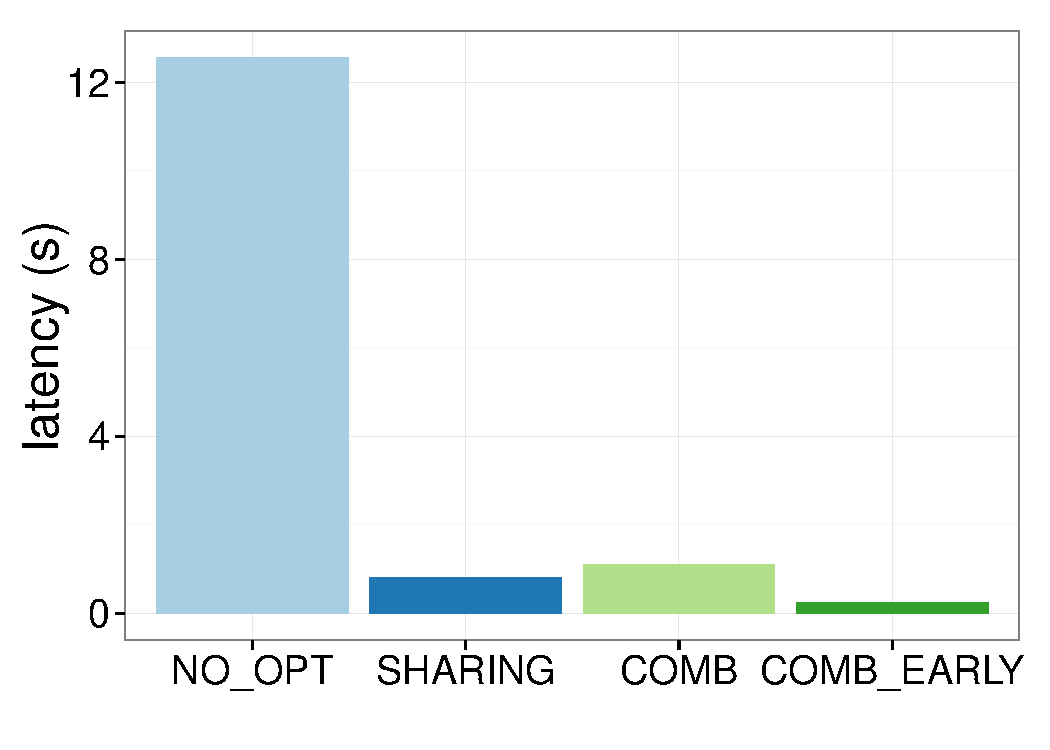
\includegraphics[width=3cm] {Images/all_opt_real_data_row_DIAB.pdf}}
% 		\caption{DIAB}
% 		\label{fig:baseline_views}
% 	\end{subfigure}
% 	\begin{subfigure}{0.24\linewidth}
% 		{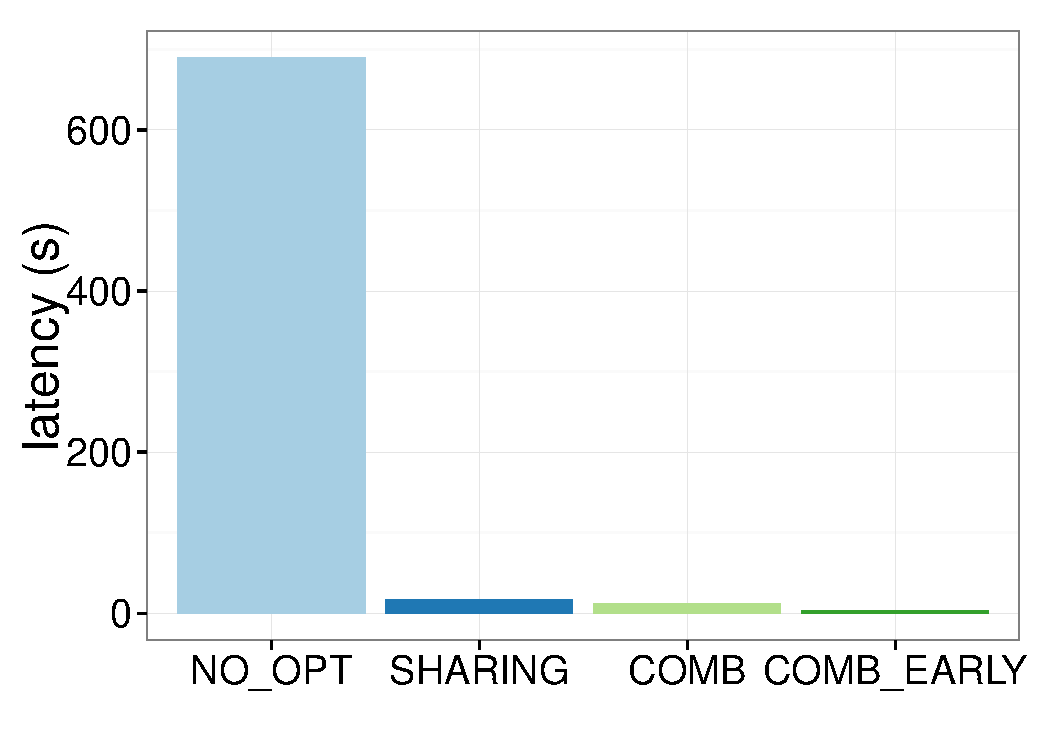
\includegraphics[width=3cm] {Images/all_opt_real_data_row_AIR.pdf}}
% 		\caption{AIR}
% 		\label{fig:multi_agg}
% 	\end{subfigure}
% 	\begin{subfigure}{0.24\linewidth}
% 		{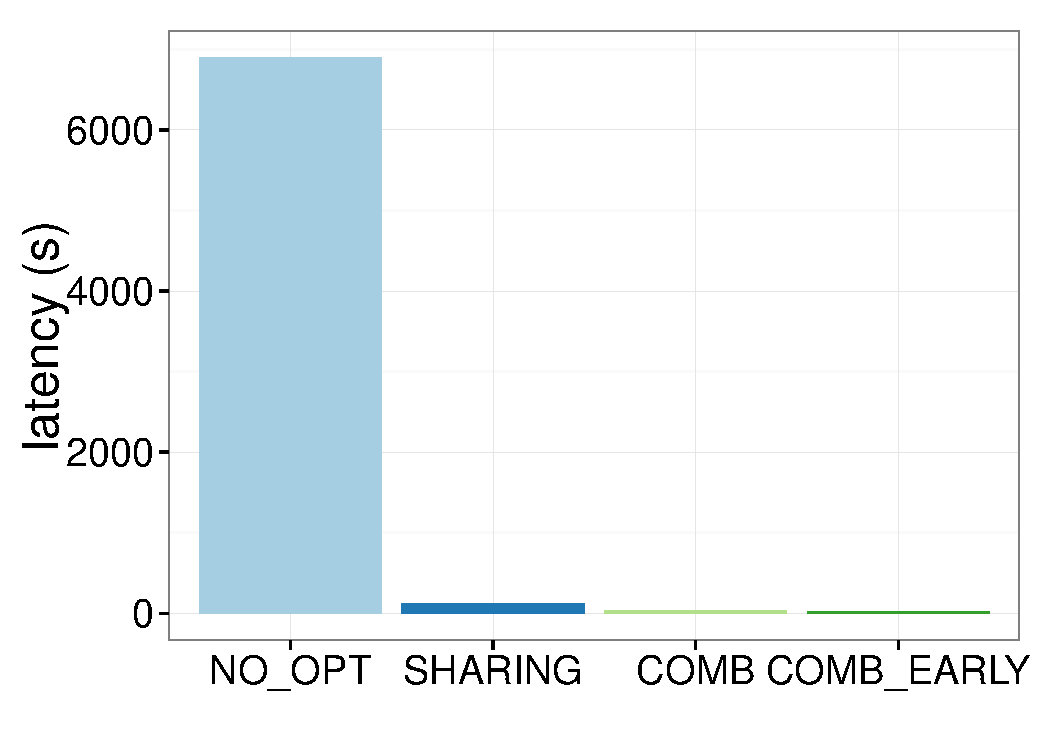
\includegraphics[width=3cm] {Images/all_opt_real_data_row_AIR10.pdf}}
% 		\caption{AIR10}
% 		\label{fig:multi_agg}
% 	\end{subfigure}
% 	\vspace{-10pt}
% 	\caption{Performance gains of all optimizations in ROW }
% 	\vspace{-10pt}
% 	\label{fig:share_prune_row}
% \end{figure}

% \begin{figure*}[t]
% 	\centering
% 	\begin{subfigure}{0.33\linewidth}
% 		\centering
% 		{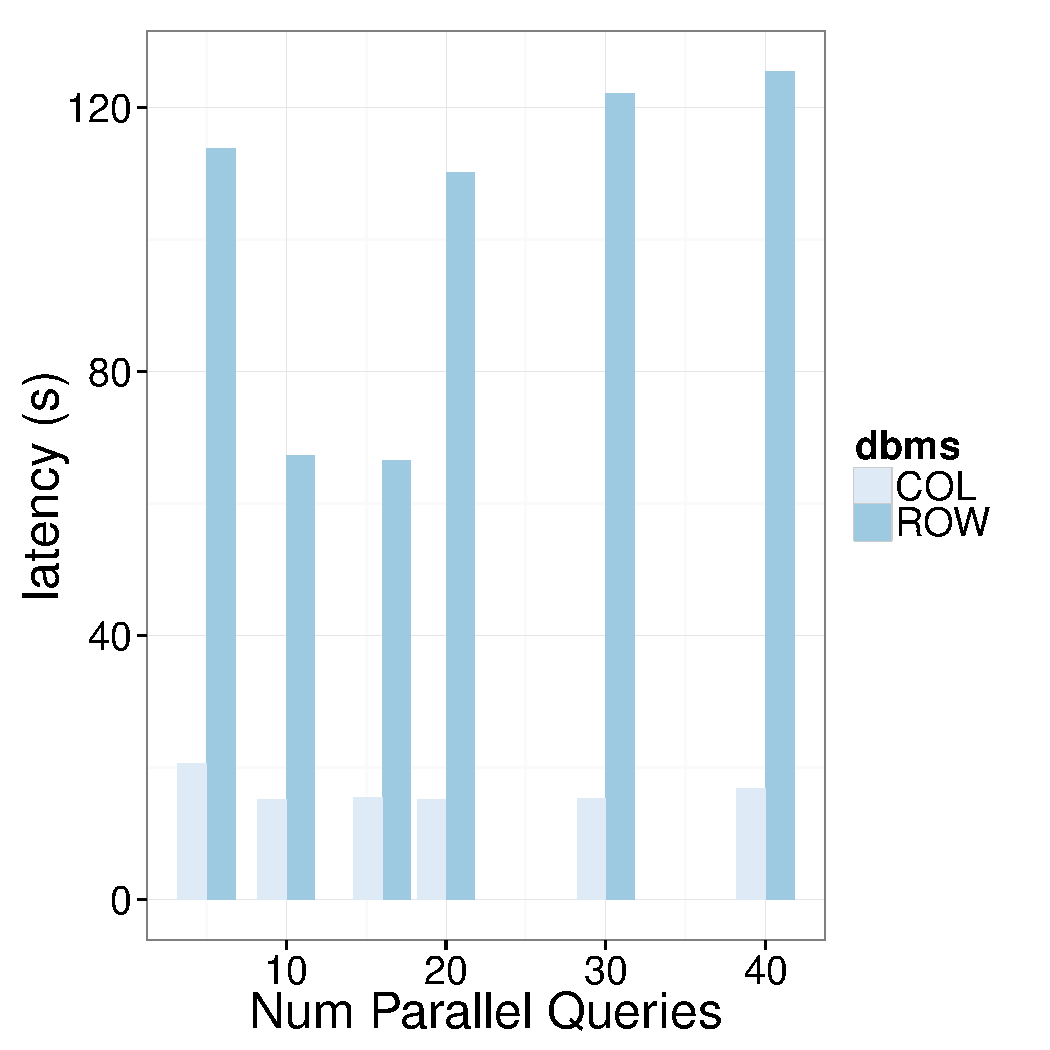
\includegraphics[width=6cm] {Images/parallel_noop.pdf}}
% 		\caption{Effect of parallelism}
% 		\label{fig:parallelism}
% 	\end{subfigure}
% 	\begin{subfigure}{0.33\linewidth}
% 		\centering
% 		{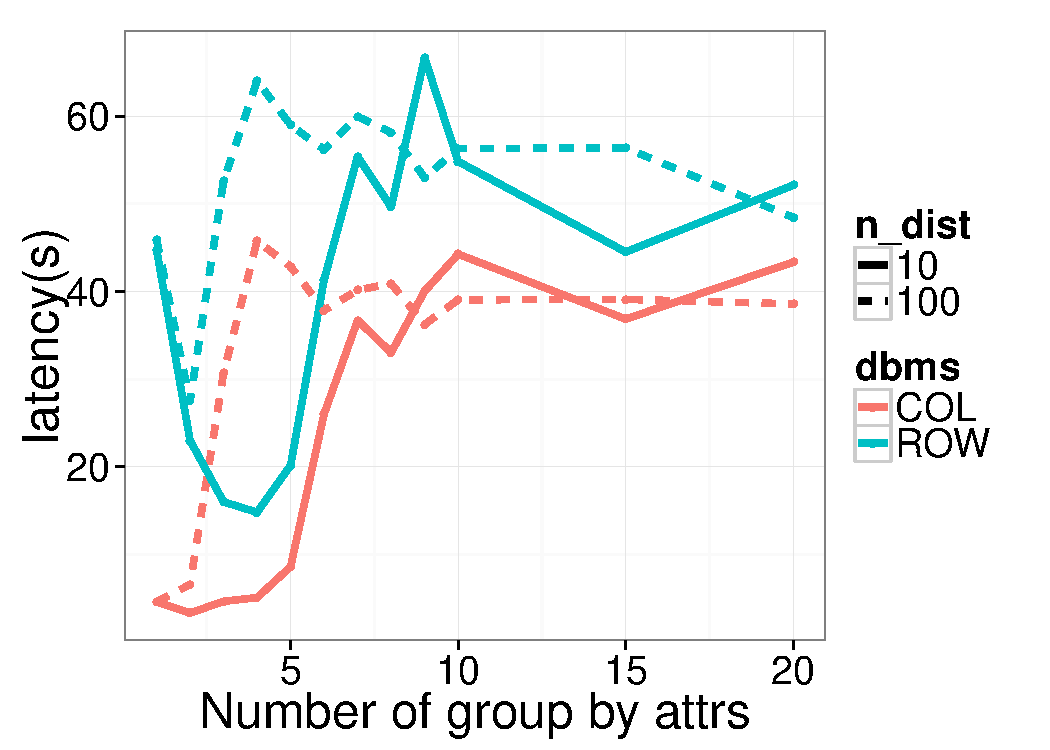
\includegraphics[width=6cm] {Images/multi_gb_same.pdf}}
% 		\caption{Latency vs. Num of Groups}
% 		\label{fig:multi_gb_same}
% 	\end{subfigure}
% 	\begin{subfigure}{0.33\linewidth}
% 		\centering
% 		{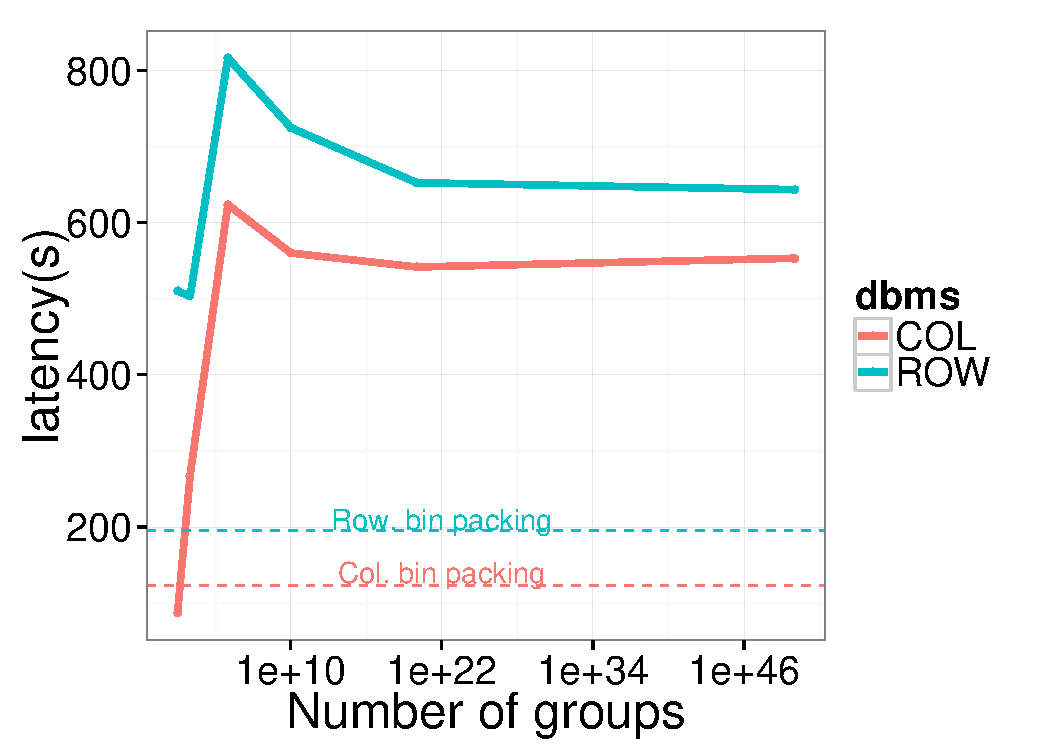
\includegraphics[width=6cm] {Images/multi_gb.pdf}}
% 		\caption{Latency vs. Num Dimensions}
% 		\label{fig:multi_gb_bp}
% 	\end{subfigure}
% 	\vspace{-10pt}
	
% 	\label{fig:bank_perf}
% 	\vspace{-10pt}
% \end{figure*}

\begin{figure}[h]
\vspace{-5pt}
	\centering
	\begin{subfigure}{1\linewidth}
		\centering
		{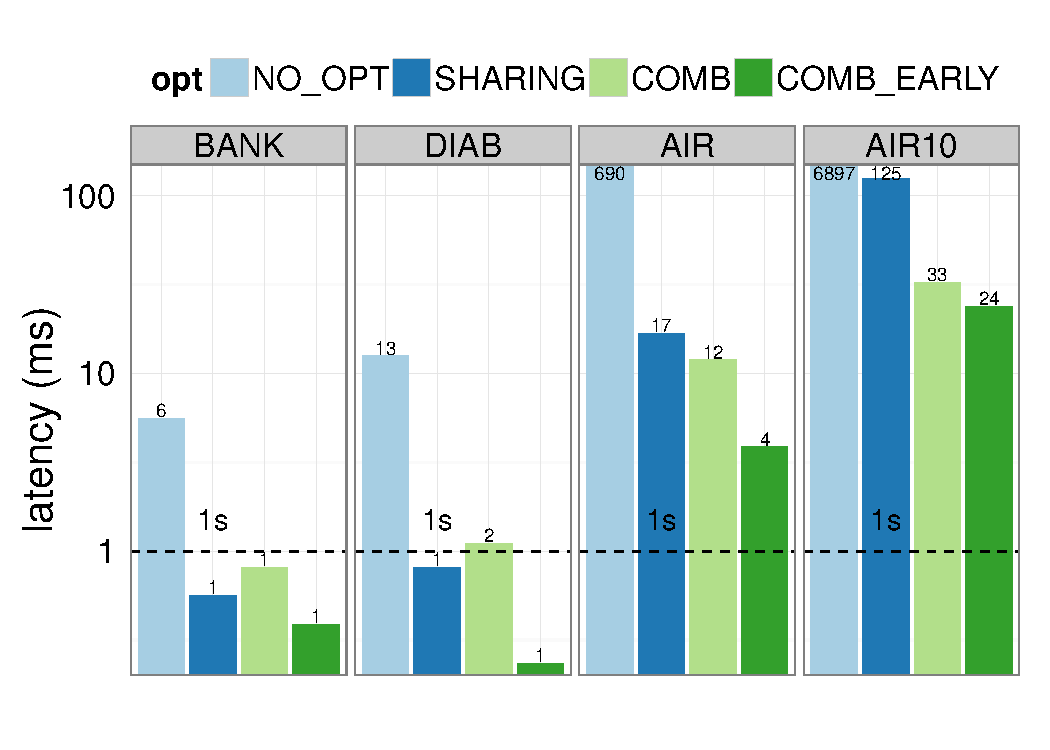
\includegraphics[width=6cm] {Images/all_opt_real_data_row.pdf}}
		\vspace{-15pt}
		\caption{Optimization results for ROW}
		\label{fig:share_prune_row}
	\end{subfigure}\\
	\begin{subfigure}{1\linewidth}
		\centering
		{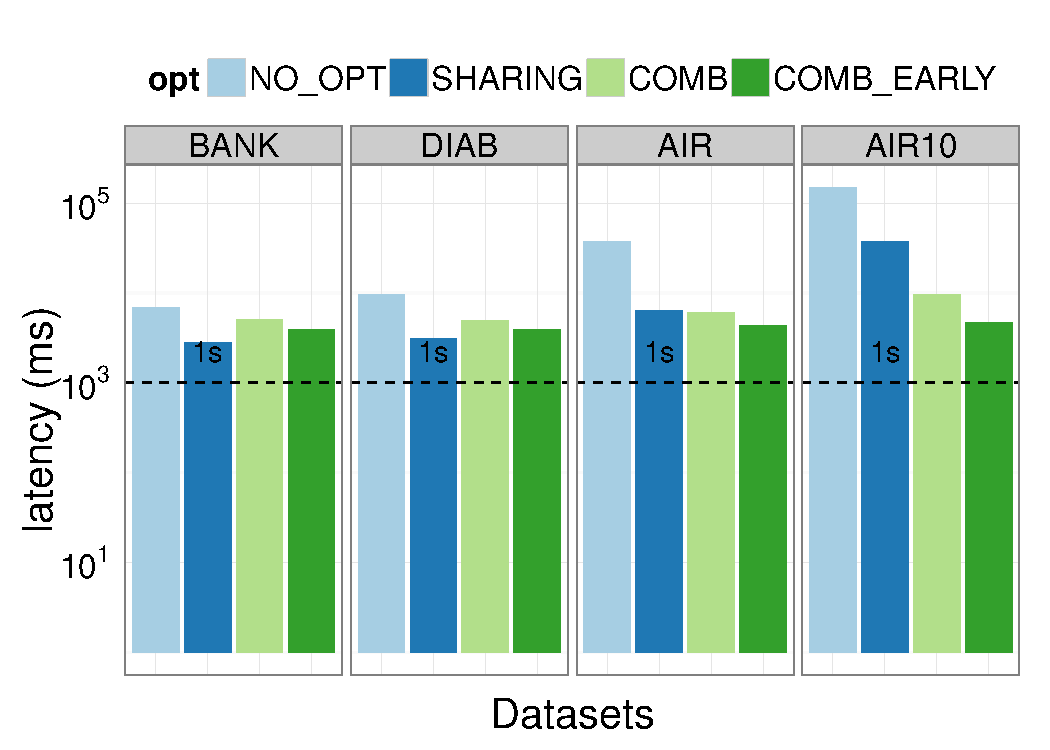
\includegraphics[width=6cm] {Images/all_opt_real_data_col.pdf}}
		\vspace{-15pt}
		\caption{Optimization results for COL}
		\label{fig:share_prune_col}
	\end{subfigure}
	\vspace{-10pt}
	\caption{Performance gains from all optimizations}
	\label{fig:all_opt_with_pruning}
	\vspace{-15pt}
\end{figure}
 
\begin{denselist} 
\item $[$\underline{\em $>$ 100X speedup overall}$]$ The combination of our sharing and pruning optimizations provides a speedup of up 
between 50X (COMB) -- 300X (COMB\_EARLY) for ROW (Figure \ref{fig:share_prune_row}) and 
10X (COMB) -- 30X (COMB\_EARLY) for COL (Figure \ref{fig:share_prune_col}).
This reduces latencies for small datasets like DIAB from 12s to 200ms, and from almost 2 hrs to tens of seconds for large datasets 
like AIR10. 
%{\it Our optimizations thus allows us to respond in real-time with exact views for small datasets and approximate views (COMB\_EARLY) for large datasets}.
\item $[$\underline{\em 8--20X speedup from sharing}$]$ The sharing optimizations (Section \ref{sec:sharing_opt}) alone produce performance gains of up to 20X for ROW and 8X for COL. 
%This enables \SeeDB to process moderate sized datasets within a few seconds.
%In fact, for small datasets like BANK and DIAB, the overheads associated with phased-execution can be avoided completely since SHARING
%alone can achieve interactive latencies.
\item $[$\underline{\em 5X speedup from pruning without loss of accuracy}$]$ Pruning optimizations (Section \ref{sec:pruning_opt}) provide additional gains of up to 5X. Early result return, in particular, enables real-time response for large datasets, e.g. for AIR, the COMB\_EARLY strategy allows \SeeDB to return results in under 4s while processing the full dataset takes tens of seconds. We also find that quality of results is not adversely affected by pruning: the utility distance (defined later) for our pruning strategies is close to 0.
\item $[$\underline{\em Multiplicative gains}$]$ A gain of 20X from sharing optimizations in the ROW store combines with the 5X gain from pruning to produce an overall gain of over 100X (Figure \ref{fig:share_prune_row}).
%\item $[$\underline{\em Column stores perform better}$]$ In general, COL stores are better suited to the \SeeDB workload and 
%significantly outperform ROW stores. The column-oriented data layout of COL enables the selective processing of specific attributes involved in each visualization. 
\item $[$\underline{\em Gains improve on larger datasets}$]$ The overall gain is much larger for AIR10 (300X) vs. BANK (10X). We find that our SHARING optimization is best suited for small datasets like BANK and DIAB, while COMB and COMB\_EARLY are essential for large datasets like AIR and AIR10.
\end{denselist}


% Thus, we conclude that the COMB and COMB\_EARLY optimizations are best suited for large datasets like AIR and AIR10 while SHARING is suitable for small datasets. 

\noindent In the next sections, we discuss the performance of individual optimizations and how they relate to the overall performance gain.



